\begin{frame}{Ejercicios}
\label{CriterioLimite}
\action<+->{
\begin{Eje}[Criterio de límite]
Encontrar el límite de la sucesión $\bigg\{n\sin\bigg(\dfrac{1}{n}\bigg)\bigg\}$
\end{Eje}}
\textcolor{red}{
\action<+->{Usando el criterio del límite:
\begin{align*}
\lim_{n\rightarrow \infty}n\sin(1/n)=&\lim_{n\rightarrow \infty}\dfrac{\sin(1/n)}{(1/n)}\\}
\action<+->{=&\lim_{n\rightarrow \infty}\dfrac{\cos(1/n)(-1/n^2)}{(-1/n^2)}\\}
\action<+->{=&\lim_{n\rightarrow \infty}\cos(1/n)\\}
\action<+->{=&1\\}
\end{align*}
\action<+->{Entonces el límite buscado es 1.\\}
}
\hyperlink{RetornoTeoremaPreliminares1}{\textcolor{cyan}{Teoremas Preliminares.}}
\end{frame}
\begin{frame}{Ejercicios}
\label{Sandwich}
\begin{Eje}[Teorema del Sandwich]
Determine el límite de la sucesión $\bigg\{\dfrac{\cos(n)}{n}\bigg\}$.
\end{Eje}
\pause
\textcolor{red}{
\begin{flalign*}
\action<+->{&-1\leq \cos(n) \leq 1\\}
\action<+->{\Rightarrow &\dfrac{-1}{n}\leq \dfrac{\cos(n)}{n} \leq \dfrac{1}{n}\\}
\action<+->{\Rightarrow &\lim_{n\rightarrow \infty}\dfrac{-1}{n}\leq \lim_{n\rightarrow \infty}\dfrac{\cos(n)}{n} \leq \lim_{n\rightarrow \infty}\dfrac{1}{n}\\}
\action<+->{\Rightarrow &0\leq \lim_{n\rightarrow \infty}\dfrac{\cos(n)}{n} \leq 0\\}
\end{flalign*}
\action<+->{Por lo tanto, el límite de la sucesión en cuestión es 0.\\}}
\hyperlink{RetornoTeoremaPreliminares1}{\textcolor{cyan}{Teoremas Preliminares.}}
\end{frame}
\begin{frame}{Ejercicios}
\label{ConvergenciaMonotona}
\begin{Eje}[Teorema de la sucesión monótona]
Encuentre el límite de la sucesión definida recursivamente por $a_n=\sqrt{1+a_{n-1}}$ con $a_1=1$, asumiendo que $\{a_n\}$ es acotada superiormente y es estrictamente creciente. 
\end{Eje}
\textcolor{red}{
\action<+->{Por el teorema de convergencia monótona existe el límite; sea $L$ tal límite, entonces:}
\begin{align*}
\action<+->{&a_n=\sqrt{1+a_{n-1}}\\}
\action<+->{\Rightarrow  \lim_{n\rightarrow \infty} &a_n=\lim_{n\rightarrow \infty}\sqrt{1+a_{n-1}}\\}
\action<+->{\Rightarrow  L=\ &\sqrt{1+L}\\}
\end{align*}
\action<+->{Resolviendo la última ecuación se obtiene que:
$$L=\dfrac{1+\sqrt{5}}{2}$$}
}
\hyperlink{RetornoTeoremaPreliminares1}{\textcolor{cyan}{Teoremas Preliminares.}}
\end{frame}
\begin{frame}{Ejercicios}
\label{EjercicioExtremos}
\begin{Eje}[Teorema de valores extremos]
Encuentre $\displaystyle\max_{x\in[2,5]}|f(x)|$ donde $f(x)=1-\exp(-\cos(x-1))$.
\end{Eje}
\textcolor{red}{
\begin{itemize}
\item \action<+->{$f$ es continua y diferenciable en [2,5].}
\item \action<+->{Por el teorema de valores extremos, existen $c_1$, $c_2$ tales que $$f(c_1)\leq f(x)\leq f(c_2),$$
para todo $x\in[2,5]$ y entonces $\displaystyle\max_{x\in[2,5]}|f(x)|= \max(|f(c_1)|,|f(c_2)|)$.}
\item \action<+->{Además dado que la función es diferenciable, se sabe que los posibles valores extremos se alcanzan en 2, 5 o donde la derivada se hace cero.$$f'(x)=\exp(-\cos(x-1))(\sin(x-1))=0.$$
Las soluciones de esta ecuación son $x=1+n\pi.$, $n\in\mathbb{Z}$. La única solución que se encuentra en el intervalo [2,5] es $x=1+\pi$. }
\end{itemize}
}
\end{frame}
\begin{frame}{Ejercicios}
\begin{itemize}
\item \action<+->{Al evaluar en los candidatos, se obtiene:
\begin{itemize}
\item $f(2)\approx 0.42$.
\item $f(5)\approx -0.92$.
\item $f(1+\pi)\approx -1.72$.
\end{itemize}
Entonces $c_1=1+\pi$ y $c_2=2$.
}
\item \action<+->{De lo anterior se obtiene que $\displaystyle\max_{x\in[2,5]}|f(x)|= \max(|f(2)|,|f(1+\pi)|)=e-1.$}
\end{itemize}
\action<+->{
\begin{figure}[H]
\begin{center}
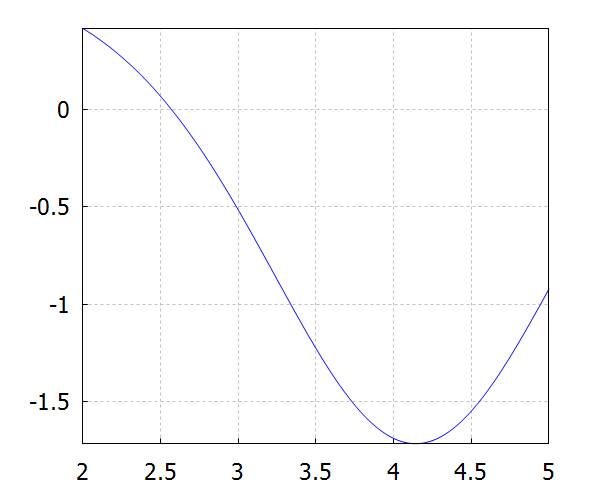
\includegraphics[scale=0.5]{Imagen16}
\end{center}
\caption{Gráfica de $f(x)$ en [2,5].}
\end{figure}}
\hyperlink{RetornoTeoremaPreliminares3}{\textcolor{cyan}{Teoremas Preliminares.}}
\end{frame}
\begin{frame}{Ejercicios}
\label{EjercicioIntermedio}
\action<+->{
\begin{Eje}[Teorema del valor intermedio]
Determine si la siguiente ecuación tiene una solución
$$\sin(x)/\log(x)=0,$$
en el intervalo $[2,4]$.
\end{Eje}}
\textcolor{red}{
\action<+->{
Elija $f(x)=\sin(x)/\log(x)$.\\ 
\indent Dado que $f(2)>0$, $f(4)<0$, $f$ es continua en [2,4] y $f(4)<0<f(2)$, entonces (tomando $K=0$) por el teorema del valor intermedio existe un $c$ tal que $f(c)=K=0$.\\}
}
\hyperlink{RetornoTeoremaPreliminares4}{\textcolor{cyan}{Teoremas Preliminares.}}
\end{frame}
\begin{frame}[fragile]{Ejercicios}
\small
\label{EjercicioBiseccion}
\begin{Eje}[Método de bisección]
Encuentre la aproximación para la solución del problema anterior usando el método de bisección. Además determine cuál es el valor de $n$ para conseguir un error de a lo mucho $10^{-5}$; calcule el error asumiendo que la solución exacta es $\pi$. ($f(x)=\sin(x)/\log(x)$, $x\in[2,4].$)
\end{Eje}
\small
\begin{lstlisting}[style=mystyle,backgroundcolor=\color{gray!30}]
n     a       b       p       f(p)            |p-p*|
0     2       4       *       *               *
1     3       4       3       1.284530e-01    1.415927e-01
2     3       3.5     3.5     -2.800077e-01   3.584073e-01
3     3       3.25    3.25    -9.179542e-02   1.084073e-01
...
16    3.1416  3.1416  3.1416  1.887677e-05    2.160867e-05
17    3.1416  3.1416  3.1416  5.547064e-06    6.349879e-06
18    3.1416  3.1416  3.1416  -1.117744e-06   1.279516e-06
19    3.1416  3.1416  3.1416  2.214656e-06    2.535182e-06
\end{lstlisting}
\normalsize
\pause
\textcolor{red}{Se necesita garantizar que $|p-\pi|\leq 10^{-5}$. Por el teorema de bisección, se tiene $$|p-\pi|\leq \dfrac{b-a}{2^n}=\dfrac{4-2}{2^n}=\dfrac{1}{2^{n-1}}\leq 10^{-5}$$
Si se resuleve la última desigualdad, se obtiene que $n\geq 17.61$, es decir que se puede escoger $n=18$.}\hyperlink{RetornoTeoremaRaices1}{\textcolor{cyan}{Raices de ecuaciones.}}
\end{frame}
\begin{frame}{Ejercicios}
\action<+->{
\begin{Eje}[Teorema de Taylor]
Considere la función $f(x)=\ln(\ln(x))$. Determine lo siguiente:
\begin{itemize}
\item Calcule $P_3(x)$ centrada en $x_0=3$.
\item Aproxime $P_3(1.5).$
\item Encuentre la expresión para $R_3(x)$.
\item Calcule el error absoluto y relativo de la aproximación anterior.
\item Aproxime $\displaystyle \int_{2}^{4}f(x)dx$ usando $P_3(x)$.
\end{itemize}
\end{Eje}
}
\label{EjercicioTaylor}
\textcolor{red}{
\begin{align*}
\action<+->{P_3(x)=&\displaystyle \sum_{k=0}^{3}\dfrac{f^{(k)}(x_0)}{k!}(x-x_0)^k\\}
\action<+->{=&\dfrac{f(3)}{0!}(x-3)^0+\dfrac{f'(3)}{1!}(x-3)^1+\dfrac{f''(3)}{2!}(x-3)^2+\dfrac{f'''(3)}{3!}(x-3)^3.}
\end{align*}}
\end{frame}
\begin{frame}{Ejercicios}
\textcolor{red}{
\begin{align*}
\action<+->{=&\ln(\ln(3))+\dfrac{(x-3)}{3\ln(3)}-\bigg(\dfrac{1}{18\ln(3)}+\dfrac{1}{18\ln^2(3)}\bigg)(x-3)^2\\
&+\dfrac{1}{162}\bigg(\dfrac{2}{\ln(3)}+\dfrac{3}{\ln^2(3)}+\dfrac{2}{\ln^3(3)}\bigg)(x-3)^3}
\end{align*}
}
\textcolor{blue}{
\begin{align*}
\action<+->{P_3(1.5)=&\ln(\ln(3))+\dfrac{(1.5-3)}{3\ln(3)}-\bigg(\dfrac{1}{18\ln(3)}+\dfrac{1}{18\ln^2(3)}\bigg)(1.5-3)^2\\
&+\dfrac{1}{162}\bigg(\dfrac{2}{\ln(3)}+\dfrac{3}{\ln^2(3)}+\dfrac{2}{\ln^3(3)}\bigg)(1.5-3)^3\\
\approx & -0.69955228}
\end{align*}
}
\textcolor{red}{
\begin{align*}
\action<+->{R_3(x)=&\dfrac{f^{(4)}(\xi(x))}{(4)!}(x-3)^{4}\\
=&-{{6\,\left(\log \xi\left(x\right)\right)^3+11\,\left(\log \xi
 \left(x\right)\right)^2+12\,\log \xi\left(x\right)+6}\over{\xi\left(
 x\right)^4\,\left(\log \xi\left(x\right)\right)^4}}(x-3)^4.
}
\end{align*}
}
\end{frame}
\begin{frame}{Ejercicios}
Observación: Si $p^*$ es una aproximación de $p$, entonces se definen los errores:
\begin{itemize}
\item Error absoluto: $|p-p^*|$.
\item Error relativo: $\dfrac{|p-p^*|}{|p|}$.
\end{itemize}
\textcolor{blue}{Error absoluto:
\begin{align*}
\action<+->{|f(1.5)-P_3(1.5)|\approx & 0.20316817}
\end{align*}
}
\textcolor{red}{Error relativo:
\begin{align*}
\action<+->{\dfrac{|f(1.5)-P_3(1.5)|}{|f(1.5)|}\approx &  0.22506211}
\end{align*}
}
\end{frame}
\begin{frame}{Ejercicios}
\textcolor{blue}{
\begin{align*}
\action<+->{\displaystyle \int_{2}^{4}f(x)dx\approx &\displaystyle \int_{2}^{4}P_3(x)dx\\}
\action<+->{=&\displaystyle \int_{2}^{4}\ln(\ln(3))+\dfrac{(x-3)}{3\ln(3)}-\bigg(\dfrac{1}{18\ln(3)}+\dfrac{1}{18\ln^2(3)}\bigg)(x-3)^2\\
&+\dfrac{1}{162}\bigg(\dfrac{2}{\ln(3)}+\dfrac{3}{\ln^2(3)}+\dfrac{2}{\ln^3(3)}\bigg)(x-3)^3 dx\\}
\action<+->{=&\bigg[\displaystyle \ln(\ln(3))(x-3)+\dfrac{(x-3)^2}{6\ln(3)}-\bigg(\dfrac{1}{54\ln(3)}+\dfrac{1}{54\ln^2(3)}\bigg)(x-3)^3\\
&+\dfrac{1}{162}\bigg(\dfrac{2}{4\ln(3)}+\dfrac{3}{4\ln^2(3)}+\dfrac{2}{4\ln^3(3)}\bigg)(x-3)^4\bigg]_{2}^{4}\\}
\action<+->{&\approx 0.1242167}
\end{align*}
}
\hyperlink{RetornoTeoremaPreliminares5}{\textcolor{cyan}{Teoremas Preliminares.}}
\end{frame}
\begin{frame}[fragile]{Ejercicios}
\label{EjercicioNewton}
\begin{Eje}[Método de Newton-Raphson,Examen I, PACI2023]
Una partícula parte del reposo sobre un plano inclinado uniforme, cuyo ángulo $\theta$ cambia con una rapidez constante de $\dfrac{d\theta}{dt}=\omega<0$.\\
Al final de $t$ segundos, la posición del objeto está dada por:
$$x(t)=-\dfrac{g}{2\omega^2}\bigg(\dfrac{e^{\omega t}-e^{-\omega t}}{2}-\sin(\omega t)\bigg)$$
Suponga que la partícula se desplazó 60 pies en 2s. Encuentre la rapidez $\omega$ con que cambia $\theta$. Asuma que $g=32.17 pies/s^2$. Para calcular dicha rapidez realice lo siguiente:
\end{Eje}
\begin{itemize}
\item\action<+->{Plantee la ecuación y determine el intervalo con extremos enteros de menor valor absoluto que contenga la solución de la ecuación.\\}
\action<+->{\textcolor{red}{Dado que $x(2)=60$, se sustituye esto en la ecuación ofrecida.}}
\end{itemize}
\end{frame}
\begin{frame}{Ejercicios}
\action<+->{\textcolor{red}{$$60=-\dfrac{g}{2\omega^2}(\sinh(2\omega)-\sin(2\omega))$$
$$120+\dfrac{g}{\omega^2}(\sinh(2\omega)-\sin(2\omega))=0$$
Defina entonces:
$$f(\omega)=120+\dfrac{g}{\omega^2}(\sinh(2\omega)-\sin(2\omega)).$$}}
\action<+->{\textcolor{red}{Dado que $\omega<0$, entonces rápidamente se puede ver que $f(-1)>0$ y $f(-2)<0$. Con esto se escoge el intervalo $[-2,-1]$.}}
\begin{itemize}
\item \action<+->{¿Cuántas iteraciones son suficientes para alcanzar una exactitud de $10^{-12}$ mediante el método de bisección?}\\
\action<+->{\textcolor{blue}{Usando el teorema de cota de error del método de bisección se plantea:
\begin{align*}
|p_n-p|\leq & \dfrac{b-a}{2^n}=\dfrac{-1-(-2)}{2^n}=\dfrac{1}{2^n}\leq 10^{-12}.\\
10^{12}\leq & 2^n.
\end{align*}
Resolviendo la inecuación se obtiene $n\geq 40$.
}}
\end{itemize}
\end{frame}
\begin{frame}[fragile]{Ejercicios}
\begin{itemize}
\action<+->{\item Realice tres iteraciones del método de bisección, calcule el error relativo en cada iteración.\\}
\action<+->{\textcolor{red}{Cuando no conocemos el valor de la raíz, la estimación del error relativo se calcula de la siguiente forma:
$$\dfrac{|p_{n+1}-p_n|}{|p_{n+1}|}$$
De esta forma se puede generar la siguiente tabla:
}
}
\end{itemize}
\pause
\small
\begin{lstlisting}[style=mystyle,backgroundcolor=\color{gray!30}]
n     a       b       p      f(p)          Error relativo
0     -2      -1      *      *             *
1     -1.5    -1      -1.5   -2.121565e+01 *
2     -1.5    -1.25   -1.25  7.755373e+00  2.000000e-01
3     -1.375  -1.25   -1.375 -6.045842e+00 9.090909e-02
\end{lstlisting}
\normalsize
\begin{itemize}
\action<+->{\item Aplique el método de Newton-Raphson para obtener una aproximación con una exactitud de $10^{-5}$. Utilice como aproximación inicial la aproximación encontrada en el iniciso anterior.}
\end{itemize}
\end{frame}
\begin{frame}[fragile]{Ejercicios}
\small
\begin{lstlisting}[style=mystyle,backgroundcolor=\color{gray!30}]
n      p_n     f(p_n)         Error relativo
0      -1.375  -6.0458        *
1      -1.3226 -1.150768e-01  3.962162e-02
2      -1.3216 -4.145716e-05  7.840103e-04
3      -1.3216 -5.371703e-12  2.826484e-07
\end{lstlisting}
\normalsize
\textcolor{blue}{Primero se requiere calcular la derivada de la función analizada:
$$f'(\omega)={{32.17\,\left(2\,\cosh \left(2\,\omega\right)-2\,\cos \left(2\,\omega\right)
 \right)}\over{\omega^2}}-{{64.34\,\left(\sinh \left(2\,\omega\right)-\sin
 \left(2\,\omega\right)\right)}\over{\omega^3}}$$
 Con esto la iteración del método de Newton queda expresado como:
 \small
 \begin{align*}
 p_{n+1}=&p_{n}-\dfrac{f(p_n)}{f'(p_n)}\\
 =&p_n+\\
 &{{3217\,p_{n}\,\sinh \left(2\,p_{n}\right)-3217\,p_{n}\,\sin
 \left(2\,p_{n}\right)+12000\,p_{n}^3}\over{6434\,\sinh \left(2\,p_{n
 }\right)-6434\,\sin \left(2\,p_{n}\right)-6434\,p_{n}\,\cosh \left(2
 \,p_{n}\right)+6434\,p_{n}\,\cos \left(2\,p_{n}\right)}}
 \end{align*}
 \normalsize
 Para los resultados se uso el error relativo, es decir $\dfrac{|p_{n+1}-p_{n}|}{|p_{n+1}|}$.\\
}
\hyperlink{RetornoTeoremaRaices4}{\textcolor{cyan}{Raices de ecuaciones.}} 
\end{frame}
\begin{frame}[fragile]{Ejercicios}
\label{EjercicioNewtonSistemas}
\begin{Eje}[Ecuaciones no lineales, Ejercicio IIPAC2023]
Sea el sistema de ecuaciones no lineales:
\begin{displaymath}
\begin{bmatrix}
\ln(x^2+y^2)-\sin(xy) &=& \ln(2)-\ln(\pi)\\
x^2+4y^2\cos(x) &=&4
\end{bmatrix}
\end{displaymath}
Realice una iteración del método de Newton Raphson para sistemas con la aproximación inicial:
\begin{displaymath}
p_0=\begin{bmatrix}
-1.5\\
-2.5
\end{bmatrix}
\end{displaymath}
Además calcule $\parallel p_k-p_{k-1}\parallel_{\infty}$ y $\parallel p_k-p_{k-1}\parallel_2$.
\end{Eje}\pause
\textcolor{red}{
Primero se definirán la función y el jacobiano para usar el método de Newton:
\small
\begin{displaymath}
F(x,y)=\begin{pmatrix}
\ln(x^2+y^2)-\sin(xy)+\ln(\pi)-\ln(2)\\
4\cos(x)y^2+x^2-4\\
\end{pmatrix}
\end{displaymath}
}
\end{frame}
\begin{frame}[fragile]{Ejercicios}
\small
\textcolor{red}{
\begin{align*}
J(x,y)=&\begin{pmatrix}
\dfrac{2x}{x^2+y^2}-y\cos(xy) & \dfrac{2y}{x^2+y^2}-x\cos(xy)\\
2x-4\sin(x)y^2 & 8 \cos(x)y 
\end{pmatrix}\\
J(-1.5,-2.5)=&
\begin{pmatrix}
 - 2.40433956981949  & - 1.819074330126988\\
 21.93737466510136   & - 1.414744033354058
\end{pmatrix}\\
J^{-1}(-1.5,-2.5)=&
\begin{pmatrix}
-0.03266761001938535 &  0.04200393103760224\\
-0.5065521278147188 &  - 0.05551818955887632
\end{pmatrix}\\
F(-1.5,-2.5)=&
\begin{pmatrix}
0.873750\\
0.018430
\end{pmatrix}\\
p_1=&p_0-J^{-1}(p_0)F(p_0)\\
=&
\begin{pmatrix}
-1.5\\
-2.5
\end{pmatrix}
-J^{-1}(-1.5,-2.5)F(-1.5,-2.5)=
\begin{pmatrix}
-1.472231\\
-2.056377
\end{pmatrix}
\end{align*}}
\small
\begin{lstlisting}[style=mystyle,backgroundcolor=\color{gray!30}]
n  p_n(1)  p_n(2)  f(p_n)        Norma 2       Norma inf
0  -1.5    -2.5    0.87375       *             *
1  -1.4722 -2.0564 -9.606503e-02 4.444916e-01  4.436233e-01
2  -1.4663 -2.1091 -1.654021e-04 5.303760e-02  5.270221e-02
3  -1.4667 -2.1087 -1.031003e-07 5.406173e-04  3.834635e-04
\end{lstlisting}
\normalsize
\hyperlink{RetornoTeoremaRaices10}{\textcolor{cyan}{Raices de ecuaciones.}} 
\end{frame}
\begin{frame}[fragile]{Ejercicios}
\begin{Eje}[Cota de error interpolación de Lagrange]
\indent Considere la siguiente función $f(x)=\sin(\ln(x)).$ Encuentre una cota para el error de aproximación del polinomio interpolante de Lagrange en el intervalo $[2,2.6]$ con tres puntos; $x_0=2$, $x_1=2.4$ y $x_2=2.6$. 
\end{Eje}
\action<+->{\ }
\begin{itemize}
\item \action<+->{\textcolor{red}{\indent Por el teorema relacionado con el polinomio de Lagrange, se sabe que:
$$|f(x)-P(x)|=\bigg|\dfrac{f^{(3)}(\xi(x))}{6}(x-2)(x-2.4)(x-2.6)\bigg|,$$
para $x\in[2,2.6]$ y $\xi(x)\in(2,2.6)$}}
\item \action<+->{\textcolor{red}{\indent Para encontrar las cotas sobre la tercera derivada se necesitan los siguientes cálculos:
\begin{align*}
f^{(3)}(z)=&\dfrac{3\sin(\ln(z))+\cos(\ln(z))}{z^3}\\
f^{(4)}(z)=&-\dfrac{10\cos(\ln(z))}{z^4}\\
\end{align*}}}
\end{itemize}
\end{frame}
\begin{frame}{Ejercicios}
\begin{itemize}
\item\action<+->{\textcolor{red}{\indent Si se analizan los lugares donde la derivada de la tercera derivada se hacen cero, entonces se obtiene la ecuación:
$$\sin(\ln(z))=0,$$
esta ecuación tiene como solución $z=e^{n\pi}$ donde $n\in\mathbb{Z}$. Para todo $n\in\mathbb{Z}$, $e^{n\pi}\notin [2,2.6]$ y por lo tanto los únicos valores extremos de la tercera derivada son 2 y 2.6.\\
\indent Evaluando la tercera derivada se obtiene que:
$$f^{(3)}(2)\approx 0.335765$$
$$f^{(3)}(2.6)\approx 0.1722$$
y por lo tanto se puede garantizar que:
$$|f^{(3)}(x)|\leq f^{(3)}(2)$$
para todo $x\in[2,2.6].$
}}
\item \action<+->{\textcolor{red}{\indent Defina ahora la otra parte para la cota de error:
$$g(x)\equiv(x-2)(x-2.4)(x-2.6)=\dfrac{25x^3-175x^2+406x-312}{25}$$
}}
\end{itemize}
\end{frame}
\begin{frame}{Ejercicios}
\begin{itemize}
\item \action<+->{\textcolor{red}{\indent Resolviendo para la ecuación de segundo grado:
$$g'(x)=0.$$
\indent Se obtiene que $x=\dfrac{35-\sqrt{7}}{15}$ (una de las dos raíces) es el lugar donde alcanza el valor más alto. Entonces:
$$|g(x)|\leq g\bigg(\dfrac{35-\sqrt{7}}{15}\bigg)$$
para toda $x\in[2,2.6]$.}}
\item \action<+->{\textcolor{red}{Finalmente:
\scriptsize
$$|f(x)-P(x)|=\bigg|\dfrac{f^{(3)}(\xi(x))}{6}(x-2)(x-2.4)(x-2.6)\bigg|
\leq g\bigg(\dfrac{35-\sqrt{7}}{15}\bigg)f^{(3)}(2)/6\approx 9.4574\times 10^{-4}$$
\normalsize
\indent La cota de error entonces es aproximadamente $9.5\times 10^{-4}$.}}
\end{itemize}
\end{frame}
%===========================
\begin{frame}{Ejercicios}
\begin{Eje}[Ejercicio del examen del IIPA2023]
Sea $f(x)=\sqrt{x-x^2}$ y $P_2(x)$ el polinomio interpolante de Lagrange en $x_0=0$, $x_1$ y $x_2=1$. Calcule el valor de $x_1$ más grande en el intervalo $(0,1)$ para el cual $f(0.5)-P_2(0.5)=-0.25$ 
\end{Eje}
\small
Tip: evalúe en los puntos desde el inicio, así se sabe que términos se cancelaran.
$$f(x_0)=f(0)=0 \quad f(x_1)=\sqrt{x_1-x_1^2}\quad f(x_2)=f(x_1)=0$$
Parte I: Determine el polinomio de Lagrange
\begin{align*}
&P_2(x)\\
&=L_0(x)f(x_0)+L_1(x)f(x_1)+L_2(x)f(x_2)\\
&=\frac{(x-x_1)(x-x_2)}{(x_0-x_1)(x_0-x_2)}f(x_0)+\frac{(x-x_1)(x-x_2)}{(x_1-x_0)(x_1-x_2)}f(x_1)+\frac{(x-x_1)(x-x_2)}{(x_2-x_0)(x_2-x_1)}f(x_2)\\
&=\frac{(x-0)(x-1)}{(x_1-0)(x_1-1)}\sqrt{x_1-x_1^2}\\
&=\frac{x(x-1)}{x_1(x_1-1)}\sqrt{x_1-x_1^2}
\end{align*}
\end{frame}
%===========================
\begin{frame}{Ejercicios}
\small
Parte 2: Evalúe en 0.5
$$P_2(0.5)=\frac{0.5(0.5-1)}{x_1(x_1-0.5)}\sqrt{x_1-x_1^2}=-\frac{0.25\sqrt{x_1-x_1^2}}{x_1(x_1-1)}$$
Parte 3: Garantizar que $f(0.5)-P_2(0.5)=-0.25$ 
\begin{align*}
f(0.5)-P_2(0.5)&=-0.25\\
0.5+\frac{0.25\sqrt{x_1-x_1^2}}{x_1(x_1-1)}&=-0.25\\
\frac{0.5+0.25}{0.25}&=\frac{\sqrt{x_1-x_1^2}}{x_1(x_1-1)}\\
-3&=\frac{\sqrt{x_1(1-x_1)}}{-x_1(1-x_1)}=-\frac{1}{\sqrt{x_1(1-x_1)}}\\
9x_1(x_1-1)&=1\\
-9x_1^2+9x_1-1&=0 \quad \implies x=\frac{1}{2}\pm\frac{\sqrt{5}}{6}
\end{align*}
Por lo tanto, \textcolor{blue}{$x_1=\frac{1}{2}+\frac{\sqrt{5}}{6}\approx 0.8726779$} 
\end{frame}
